\section{Numerical Results}
\label{sec:numerical}

In order to turn the BIEs analyzed
above into discrete linear systems,
we require some standard techniques
from the BIE literature.

Let the boundary be divided into $N_p$
panels.
%
We parameterize panel $j$ as
$\bx_j(t)$, with $t$ ranging over the
interval $[-1,1]$.
%
Each component of $\bx_j$ is taken to be
a polynomial interpolant over the
standard 16th order Legendre nodes on
$[-1,1]$, denoted by $t_n$, so that
the total number of discretization
points is $N=16N_p$.
%
See \cref{fig:panels} for an example
discretization.
%
Another important quantity below is the
arc-length density of a panel, which
we denote by $s_j(t) := |\bx'_j(t)|$.
%
Finally, we denote the set of panels
which are adjacent to panel $i$
by $A(i)$. On a closed curve,
$A(i)$ contains two integers.

The integral kernels of the single and
double layer potentials have weak
singularities of the form $r^p\log r$
which require special quadrature rules to
achieve high-order accuracy.
%
In the examples below, we use generalized
Gaussian quadrature (GGQ)~\cite{bremer2010}.
%
To demonstrate the idea, we consider
evaluating the convolution of a kernel
$K$ with a density $\sigma$
at the boundary node $\xx_j(t_l)$.
%
GGQ is a Nystr\"{o}m-type discretization ---
the density is approximated 
by its values at the discretization nodes,
which we denote by
$\sigma_{qp} \approx \sigma(\xx_q(t_p))$.
%
The basis of a GGQ rule is a set of 
support nodes and weights for the
contribution to the integral from the
``self'' panel (panel $j$) and the adjacent
panels (with index in $A(j)$).
%

For the self panel, there is a special set
of nodes and weights for each interpolation
point. Denote the nodes and weights
for interpolation point $l$ by $t^{(l)}_{n}$
and $w^{(l)}_{n}$, respectively, with
$1\leq l \leq 16$ and $1\leq n \leq N_s$.
%
The adjacent panels are handled by a single
set of over-sampled support nodes and weights.
We denote these nodes and weights
by $\tilde{t}_n$ and $\tilde{w}_n$, respectively,
for $1 \leq n \leq N_a$.
%
For the rules we used, $N_s = 16$ and
$N_a = 48$.
%
The contribution of other panels is assumed
to be given to high accuracy by the standard
Gauss-Legendre weights, which we denote
by $w_n$.
%
Adding these contributions together, we obtain the
quadrature

\begin{multline}
  \int_\Gamma K(\xx_i(t_l),\yy) \, \sigma(\yy)
  \, dS(\yy) \approx \\
  \sum_{p=1}^{16} \sum_{n=1}^{N_s}
  w^{(l)}_{n} K(\xx_i(t_l),\xx_i({t}^{(l)}_{n}))
  s_i({t}^{(l)}_{n}) B^{(l)}_{np} \sigma_{ip} \quad \textrm{(self)}
  \\
  + \sum_{q\in A(i)} \sum_{p=1}^{16} \sum_{n=1}^{N_a}
  \tilde{w}_jK(\xx_i(t_l),\xx_q(\tilde{t}_n)) s_q(\tilde{t}_n)
  C_{np} \sigma_{qp}
  \quad \textrm{(adjacent)} \\
  + \sum_{q\neq i, q\not\in A(i)} \sum_{p=1}^{16}
  w_p K(\xx_i(t_l),\xx_q(t_p)) s_q(t_p)
  \sigma_{qp} \quad \textrm{(far)} \nonumber \; ,
\end{multline}
where $\bB^{(l)}$ and $\bC$ are interpolation
matrices from the standard Legendre nodes
to the self and adjacent panel support nodes,
respectively. Observe that the quadrature is
linear in $\sigma_{qp}$. In practice, we pre-compute
and store the self and adjacent matrix entries for each
interpolation point, which is a parallelizable
$O(N)$ calculation. The ``far'' interactions
are computed on-the-fly.

Once the discretization is set, we can form
a compressed representation of the system matrix
using recursive skeletonization~\cite{ho2012fast}.
%
We use the implementation of this procedure
included in the fast linear algebra in
MATLAB (\texttt{FLAM}) package
\cite{hoFLAM_1253582}.
%
At low-to-medium frequencies, the scaling
of the recursive skeletonization algorithm
is $O(N\log N)$ in operation count and
storage and, by using a generalization
of the Sylvester determinant formula,
allows for a fast determinant
calculation in $O(N\log N)$ time as a
follow-up step.
%
At higher-frequencies,
the recursive skeletonization procedure,
which is based on the assumption that off-diagonal
blocks of the matrix are of low rank,
breaks down and does not offer a speed advantage.
%
These algorithms take a precision parameter
$\epsflam$ which determines the
accuracy to which any sub-blocks of the matrix
should be compressed. In all experiments,
we set $\epsflam = 10^{-14}$.

To estimate the eigenvalues, we fit a Chebyshev
interpolant to the discretized determinant as a
function of $k$ on intervals.
%
This is done adaptively so that the Chebyshev
coefficients of the determinant have decayed
to the point that the ratio of the last
coefficient to the largest coefficient is below
some threshold.
%
In all experiments, we set this threshold
as $\epscheb = 10^{-13}$.
%
We perform this fit using the \texttt{chebfun}
utility in the package of the same name
\cite{driscoll2014chebfun}
so that we can make use
of the \texttt{roots} utility to approximate
the roots of the determinant.

Below, we let $D^N_k$, $S^N_k$ and $W^N$ denote
the discretized versions of the $\cDk$,
$\cSk$, and $\cW$ operators, respectively.



\subsection{Eigenvalues of an annulus}

\subsubsection{Spurious eigenvalues}
\label{subsec:spurannulus}



\subsubsection{Convergence study}
\label{subsec:convannulus}

\subsection{Eigenvalues of a barbell-shaped domain}
\label{subsec:barbell}

\begin{figure}
  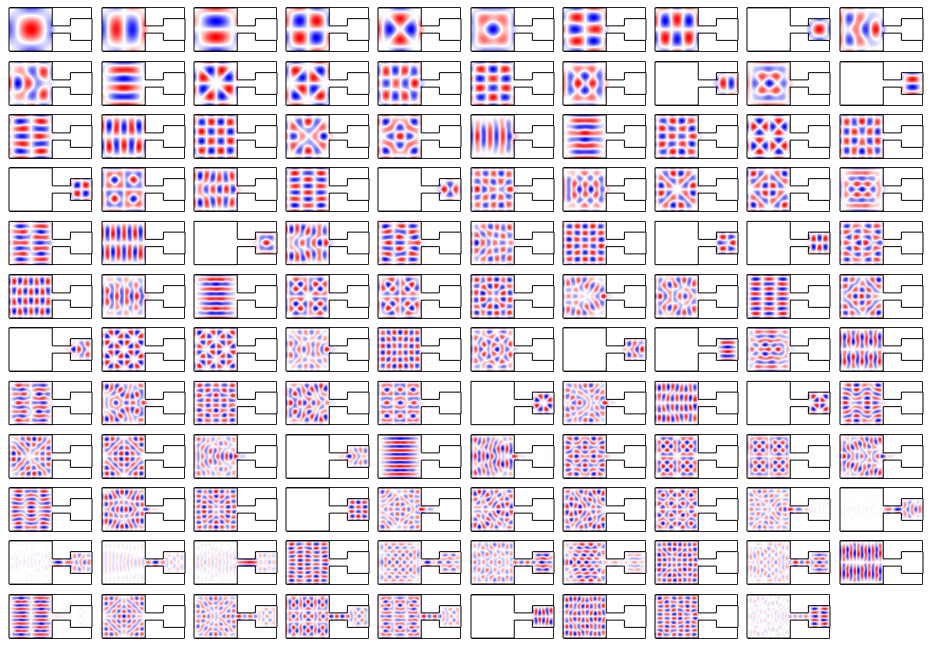
\includegraphics[width=\textwidth]{fig/barbell_gallery}
  \caption{Vorticity plots of the first 110 eigenfunctions
    of the barbell-shaped domain.}
  \label{fig:barbell_gallery}
\end{figure}

%\subsection{Robustness on a nearly multiply connected domain}
%\label{subsec:crescent}

\subsection{Eigenvalues of a domain with several inclusions}

